\section{Lecture 13: The Sampling Theorem}

Consider the task of sampling an analog signal, which presents
us with a discrete signal. This process is referred to as \textbf{sampling}.
Discretising in time is very much an ``$x$-axis problem'', but there's
also a complementary ``$y$-axis'' problem where the values of a signal cannot
be sampled with infinite precision -- this is referred to as
\textbf{quantisation} and will be discussed in a later lecture.

\subsection{Periodic Sampling}
%
A discrete-time signal is acquired by sampling a continuous-time signal
each $T$ units, i.e.
%
\begin{displaymath}
  x[n] = x_c(nT) \,,
\end{displaymath}
%
where $n$ is an integer and $T$ is referred to as the \textbf{sampling period}.
The derived parameter $\omega_s=\frac{2\pi}{T}$ is the
\textbf{sampling frequency}, measured in radians (alternatively in Hz,
the sampling frequency is $\frac{1}{T}$). Of course, there's no way to
sample the value of an analog signal at a time with infinite resolution;
what happens in reality is that the signal is averaged over some small
interval, which introduces some noise into the measurement process. Our
measured signal is then $x_c(t) * h(t)$, where $h(t)$ is some window function
of finite duration corresponding to the impulse response of the sampler.
There may be other sources of noise in the system, meaning our discrete-time
signal becomes
%
\begin{displaymath}
  x[n] = x_c(t) * h(t) + z[n] \,,
\end{displaymath}
%
where $z[n]$ denotes some noise process. For the moment, we're going to
assume that our sampling is ideal, and our only question is how to recover
the continuous-time signal from a discretely sampled signal.

\subsection{Reconstruction of an Analog Signal}
%
The faithful reconstruction of $x_c(t)$ from $x[n]$ is clearly not possible
as it describes a one-to-many problem; we cannot simply eliminate information
from the description of a signal (i.e. those values $x_c(nT + \delta t)$ to
$x_c((n+1)T - \delta t)$) and expect to recover them. There are a number of
simple estimates that we can use to infer those values of the analog signal
which we're sampled. These strategies are depicted in Figure
\ref{fig::lecture_13_interpolation_filters}. Note that neither the nearest
neighbor or linear interpolation impulse responses are causal.\\
%
\begin{figure}[!htb]
  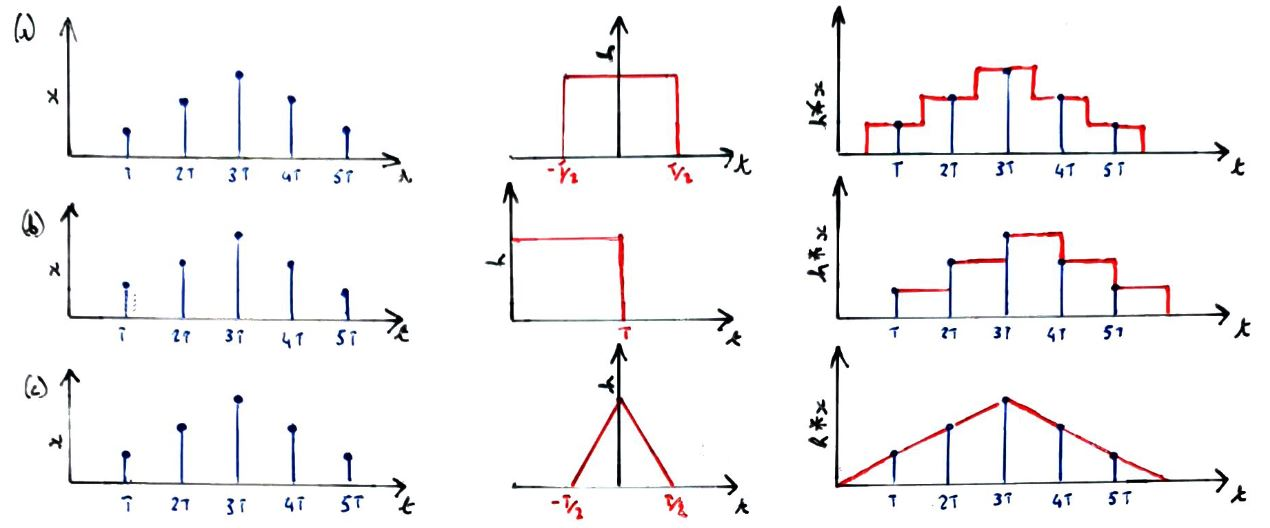
\includegraphics[width=\textwidth]{images/lecture_13_interpolation_filters.JPG}
  \caption{
  }
  \label{fig::lecture_13_interpolation_filters}
\end{figure}
%
A motivating example for why we need to be careful with our sampling of
an analog signal is given in Figure \ref{fig::lecture_13_aliasing}. Consider the sinusoid drawn in
black, whose frequency is higher than the sampling frequency (1.5 cycles
of the sinusoid elapse between discrete samples). Performing a smooth
interpolation of our discrete signal then recovers a sinusoid whose frequency
is lower than that which we originally sampled. We must place some
restrictions on our input signal so that we're not met with these types
of problem. A restriction that we'll find useful is that of a
\textbf{band-limited} signal, whereby there is some frequency $\omega_B$
such that
%
\begin{displaymath}
  X_c(\omega) = 0,\quad |\omega| > \omega_B \,.
\end{displaymath}
%
\begin{figure}[!htb]
  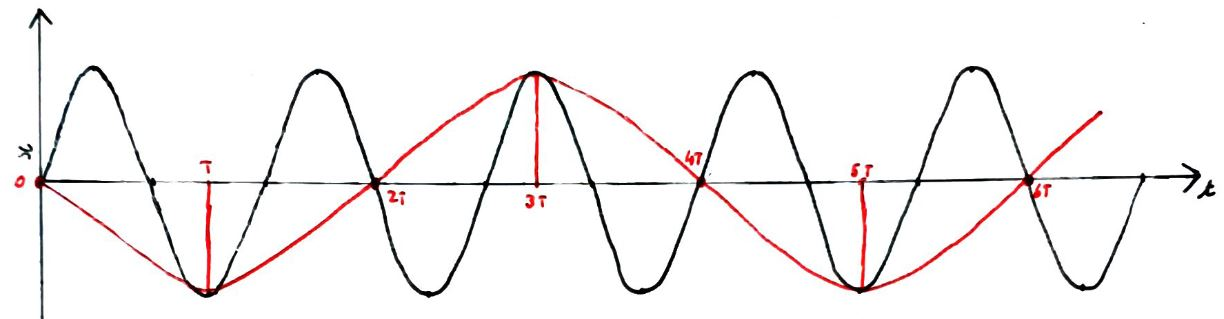
\includegraphics[width=\textwidth]{images/lecture_13_aliasing.JPG}
  \caption{
  }
  \label{fig::lecture_13_aliasing}
\end{figure}
%

\subsection{The Shannon-Nyquist Sampling Theorem}
%
A band-limited signal with maximum frequency $\omega_B$ can be perfectly
reconstructed from evenly-spaced samples if the sampling frequency
$\omega_s$ satisfies
%
\begin{equation}
  \omega_s > 2\omega_B \,,
\end{equation}
%
where $2\omega_B$ is referred to as the \textbf{Nyquist rate}.\\

Consider the act of sampling a continuous-time signal. This can be
written as the multiplication of the signal with an impulse train,
%
\begin{displaymath}
  x_s(t) = x(t) h(t) \,,
\end{displaymath}
%
where $x_s(t)$ is also a continuous-time signal which resembles
$x[n]$. We previously saw that for an impulse train, the Fourier
transform is given by $\frac{1}{T}$ for all spectral coefficients.
QQ Make sure this derivation is given in full.
Since we're working in radians, this becomes $\frac{2\pi}{T} = \omega_s$,
the separation between impulses being at $\frac{2\pi n}{T}$. As such,
%
\begin{displaymath}
  x_s(t) = x_c(t) h(t) \quad\Longleftrightarrow\quad
  X_s(\omega) = \frac{1}{2\pi}X_c(\omega) * H(\omega) \,.
\end{displaymath}
%
Note the factor of $\frac{1}{2\pi}$; this is to normalise the expression
for the Fourier transform of a periodic signal that we've previously
encountered,
%
\begin{displaymath}
  X(\omega) = \infsum{k}2\pi a_k\delta(\omega-k\omega_0) \,.
\end{displaymath}
%
Now, expanding out the frequency response,
%
\begin{displaymath}
  X_s(\omega) = \frac{1}{2\pi}X_c(\omega) * \left[
    \frac{2\pi}{T}\infsum{k}\delta(\omega - k\omega_s)
  \right] = \frac{1}{T}\infsum{k} X_c(\omega-k\omega_s) \,.
\end{displaymath}
%
Graphically (see Figure \ref{fig::lecture_13_nyquist}),
this means that $X_c(\omega)$ is scaled by
$\frac{1}{T}$ and duplicated each $k\omega_s$ units on the frequency axis.
Now, since the signal is band-limited, we see that the condition
$\omega_s - \omega_B > \omega_B \Longrightarrow \omega_s > 2\omega_B$
ensures that duplicates never overlap, and hence the inequality which
defines the sampling theorem.\\
%
\begin{figure}[!htb]
  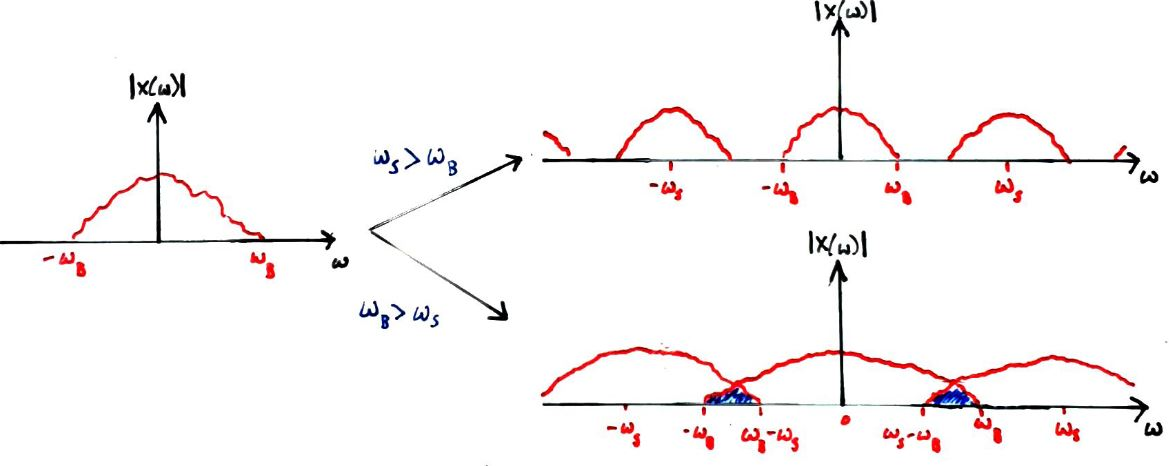
\includegraphics[width=\textwidth]{images/lecture_13_nyquist.JPG}
  \caption{
  }
  \label{fig::lecture_13_nyquist}
\end{figure}
%
To reconstruct our original analog signal $x_c(t)$, we need simply scale
$X_s(\omega)$ by $T$ and use a low-pass filter to remove all duplicates.
This means our reconstruction filter, $H_r(\omega)$, is a top hat function
on $\left[-\frac{\omega_s}{2},\frac{\omega_s}{2}\right]$ (or any shorter
duration) and height $T$. Inverse Fourier transforming then returns $x_c(t)$.
Any overlapping of duplicates in the frequency domain would result in higher
frequencies being combined with lower frequencies of copies, a phenomenon
referred to as \textbf{aliasing}. Note that while the CTFT is
$\omega_s$-periodic, the DTFT is $2\pi$-periodic, so replicas of $X(\omega)$
would be situated $2\pi$ apart on the frequency axis. The bandlimit, $\omega_B$
would be similarly scaled to appear at $\frac{2\pi\omega_b}{\omega_s} = \omega_B T$.\\

Thinking about this in the time domain, given $H_r(\omega)$ is
$T\rect{\omega/\omega_s} = T\rect{\omega T/2\pi}$, the impulse response
must be $h_r(t) = \sinc\left(\frac{\pi t}{T}\right)$, a $\sinc$ whose zeroes
are at integer multiples of $T$. The time-domain signal we recover from the sampled
signal is then
%
\begin{displaymath}
  x(t) = x_s(t)*h_r(t) = \infsum{n} x[n]\sinc\left(\frac{\pi}{T}(t - nT)\right) \,.
\end{displaymath}
%
It's worth considering what this infinite sum of shifted sinc functions looks
like. It is graphed in Figure \ref{fig::lecture_13_sincs}.
At each discretely sampled point, a sinc
function is centred, but all other sincs in the summation are zero at integer
multiples of $T$. The values of $x(t)$ between integer multiples of $T$ are
given by the summation over an infinite number of sinc functions at that point.
%
\begin{figure}[!htb]
  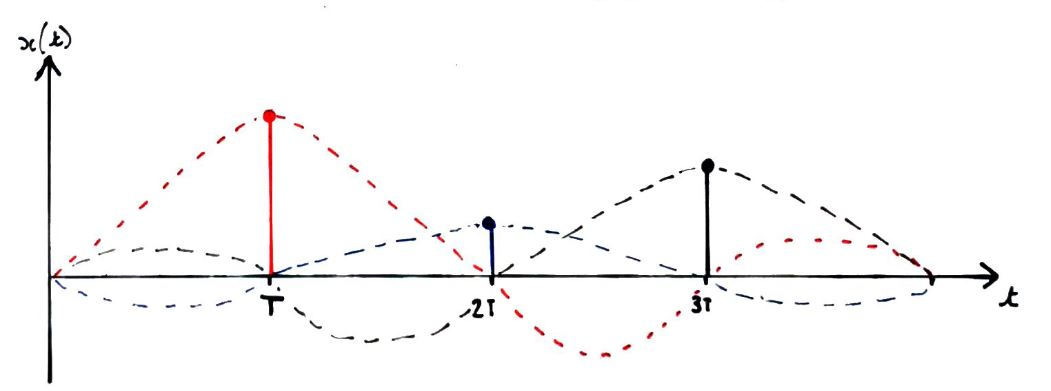
\includegraphics[width=\textwidth]{images/lecture_13_sincs.JPG}
  \caption{
  }
  \label{fig::lecture_13_sincs}
\end{figure}
%
\begin{exmp}
  Consider a cosine and its Fourier transform
  %
  \begin{displaymath}
    x(t) = \cos(\omega_0 t) \quad\Longleftrightarrow\quad
    X(\omega) = \delta(\omega+\omega_0) + \delta(\omega-\omega_0) \,.
  \end{displaymath}
  %
  The sampling theorem tells us that to avoid aliasing, we must choose
  a sampling frequency that is greater than $2\omega_0$; an example of this
  is given in Figure QQ. However, consider the case where $\omega_0=1$ and
  $\omega_s = 3/2$ as depicted in Figure \ref{fig::lecture_13_aliasing_cosine}.
  Since $\omega_s < 2\omega_0$, we observe the creation of frequencies at
  $\pm\frac{1}{2}$. Since the reconstruction filter cutoff is
  $\omega_s/2 = 3/4$, the reconstructed signal is $\cos(\frac{1}{2}t)$; aliasing
  produces the wrong result.
  %
  \begin{figure}[!htb]
    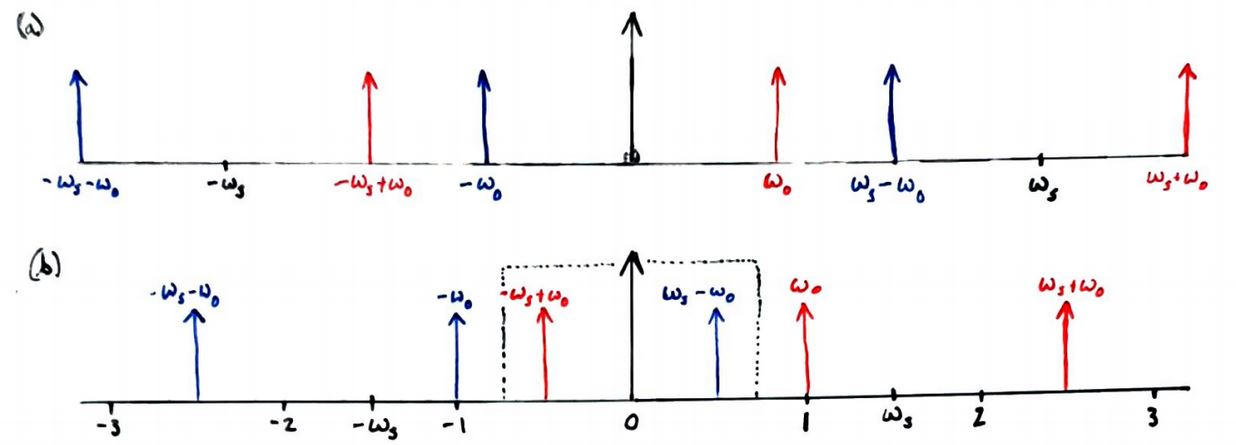
\includegraphics[width=\textwidth]{images/lecture_13_aliasing_cosine.JPG}
    \caption{
    }
    \label{fig::lecture_13_aliasing_cosine}
  \end{figure}
  %
\end{exmp}
%
\begin{exmp}
  Consider $\cos(\omega_0 t)$, where $\omega_0 = 1$ and $\omega_s = 2$,
  precisely twice the highest frequency component of the signal. The sampling
  period is $T = 2\pi / \omega_s = \pi$, meaning we sample the signal at
  integer multiples of $\pi$. For the cosine, this yields sampled values of
  $\pm 1$, so it seems that we can sample a cosine at the Nyquist rate with
  no issue.\\
  %
  However, consider now $\sin(\omega_0 t)$, parameterised in the same way as
  above. Sampling this signal at integer multiples of $\pi$ yields zero each
  time, and we're unable to recreate our original signal. Hence the reason
  that the sampling rate should be \textbf{above} the Nyquist rate, to
  accommodate this worst-case scenario.
\end{exmp}
